% !TEX TS-program = pdflatex
% !TEX encoding = UTF-8 Unicode  

% This is a simple template for a LaTeX document using the "article" class.
% See "book", "report", "letter" for other types of document.

\documentclass[11pt]{article} % use larger type; default would be 10pt

\usepackage[utf8]{inputenc} % set input encoding (not needed with XeLaTeX)

%%% Examples of Article customizations
% These packages are optional, depending whether you want the features they provide.
% See the LaTeX Companion or other references for full information.

%%% PAGE DIMENSIONS
\usepackage{geometry} % to change the page dimensions
\geometry{a4paper} % or letterpaper (US) or a5paper or....
\geometry{margin=0.8in} % for example, change the margins to 2 inches all round
% \geometry{landscape} % set up the page for landscape
%   read geometry.pdf for detailed page layout information

\usepackage{graphicx} % support the \includegraphics command and options
\usepackage{floatrow}
\usepackage{multirow}
\usepackage{url}

\usepackage[svgnames]{xcolor}
\usepackage{listings}

\lstset{language=R,
    basicstyle=\small\ttfamily,
    stringstyle=\color{DarkGreen},
    otherkeywords={0,1,2,3,4,5,6,7,8,9},
    morekeywords={TRUE,FALSE},
    deletekeywords={data,frame,length,as,character},
    keywordstyle=\color{blue},
    commentstyle=\color{DarkGreen},
}


% \usepackage[parfill]{parskip} % Activate to begin paragraphs with an empty line rather than an indent

%%% PACKAGES
\usepackage{booktabs} % for much better looking tables
\usepackage{array} % for better arrays (eg matrices) in maths
\usepackage{paralist} % very flexible & customisable lists (eg. enumerate/itemize, etc.)
\usepackage{verbatim} % adds environment for commenting out blocks of text & for better verbatim
\usepackage{subfig} % make it possible to include more than one captioned figure/table in a single float
% These packages are all incorporated in the memoir class to one degree or another...

%%% HEADERS & FOOTERS
\usepackage{fancyhdr} % This should be set AFTER setting up the page geometry
\pagestyle{fancy} % options: empty , plain , fancy
\renewcommand{\headrulewidth}{0pt} % customise the layout...
\lhead{}\chead{}\rhead{}
\lfoot{}\cfoot{\thepage}\rfoot{}

%%% SECTION TITLE APPEARANCE
\usepackage{sectsty}
\allsectionsfont{\sffamily\mdseries\upshape} % (See the fntguide.pdf for font help)

% (This matches ConTeXt defaults)

%%% ToC (table of contents) APPEARANCE
\usepackage[nottoc,notlof,notlot]{tocbibind} % Put the bibliography in the ToC
\usepackage[titles,subfigure]{tocloft} % Alter the style of the Table of Contents
\renewcommand{\cftsecfont}{\rmfamily\mdseries\upshape}
\renewcommand{\cftsecpagefont}{\rmfamily\mdseries\upshape} % No bold!

%%% END Article customizations

%%% The "real" document content comes below...

\title{\vspace{-0cm}Introduction to Machine Learning Assessment}
\author{Michael Hoskin}
\date{} % Activate to display a given date or no date (if empty),
         % otherwise the current date is printed 

\begin{document}

\vspace{-5mm}
\maketitle

\section{Introduction}


\subsection{Classification Problems}

Within machine learning, a classification problem an example of supervised learning, where labelled training data is used to attempt to classify unlabelled data, rather than just attempting to cluster data into homogeneous groups. 

For training observations $X$, with labels $Y$, we try to find a function $f : x \rightarrow y$, so that for an unknown observation, $f(x)$ can predict with a high success rate the output $y$.

K-Nearest-Neighbours (kNN) is a simple but powerful classification algorithm. It is non-parametric, in that it makes no explicit assumptions about the form of $f$ and avoids the risk of attributing an incorrect distribution to the data. It is also instance-based, in that it doesn't create or learn a model, instead the only output of running a kNN on a data set is a an array of predicted values to compare with the data's actual values. As the algorithm must store the entire data set in memory, there is both a large memory cost, and a large processing cost as the entire data set must be iterated over for each observation. 

Within the kNN algorithm, k must be chosen in advance. A very small k provides a flexible fit, but removes knowledge of overall distributions of points. A higher k however is more resilient to outlying data points, and will have smoother boundaries. 

\subsection{Training and Test Data Sets}

For classification problems, data sets are usually split into two: a training set and a test set.

The classifier is initially built using the training data, which contains both input data to pass to the classifier, and corresponding output values.

The test data is used once a model has been created, to test classifier performance on an independent dataset. If a classifier can fit the test data, it can be considered relatively free of overfitting. There should be no overlap between training and test data sets. 


\subsection{Introduction to MNIST}

The MNIST (Modified National Institute of Standards and Technology) database is a database of handwritten digits, and consists of 70,000 images, pre-split into 60,000 training images, and 10,000 test images, and is commonly used to test classification techniques as it is well structured and preprocessed. An example digit can be found in Figure \ref{fig:mnist_example}.



\begin{figure}[htb!]
\floatbox[{\capbeside\thisfloatsetup{capbesideposition={right,center},capbesidewidth=9cm}}]{figure}[\FBwidth]
{\caption{Example MNIST image denoting the digit '5', refactored from 1x784 to 28x28.}\label{fig:mnist_example}}
{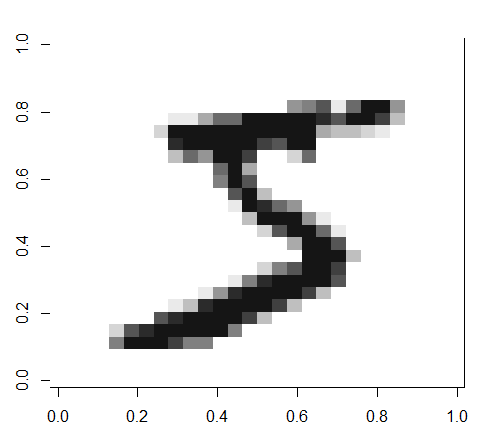
\includegraphics[width=0.15\textwidth]{mnist_example.png}}
\end{figure}

Each digit comes in the form of a 28x28 array of numbers between 0 and 255, representing a greyscale range. The digits have been size-normalised and centered. The data set as a whole originates from a much larger data set taken from NIST's (National Institute of Standards and Technology) Special Database 1 (SD-1) and Special Database 3 (SD-2). 30,000 images from each were selected to form the training set, and 5,000 of each selected to form the test set. SD-1 consists of digits written by high-school students, while SD-3 consists of digits written by employees of the US Census Bureau, and thus are cleaner and easier to recognise than SD-1 digits. The split of digits into training and test was chosen to ensure that there is no overlap of author between the training and test sets - a random author will have digits in either the training data, or the test data, but not both. \cite{mnist-website}



\section{Dimensionality Reduction}

With the original MNIST data set, we can consider each observation to have 784 dimensions - one for each of the 28 x 28 pixel values, ranging from 0 to 255. If we can reduce this to a number of key dimensions, we can remove variables with minimal variance - such as the corners - and reduce processing time as there is less data to compute distances for.

Principal Component Analysis (PCA) is a common method of dimensionality reduction.It can be thought of fitting an n-dimensional ellipsoid to a set of n dimensional data, where a long axis represents a feature with high variance. Principal components (PCs) are new properties constructed from the original features which can be used to summarise data; keeping only the first principal components retains most of the key information for classifying data. 

 Figure \ref{fig:pca_rotations_range} shows Eigenvalues relating to PCs 1 to 5, 101 to 105, and 780 to 784. While the first 5 can be recognised as numbers, the second set of 5 appear to be just noisy ovals, while the last set of 5 have very little meaningful data.  Figure \ref{fig:cumsum_pca} shows a cumulative plot revealing that 87 PCs are enough to retain 90\% of the raw information. Diminishing returns occurs, so considering another 87 PCs increases this to only 95.8\%. 

%\begin{figure}[htb!]
%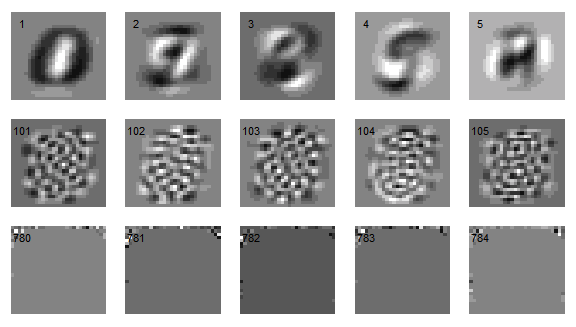
\includegraphics[width = 0.8\textwidth]{pca_rotations_wider_range.png}
%\caption{Eigenvectors 1 to 5 (top), eigenvectors 101 to 105 (middle), and eigenvectors 780 to 784 (bottom). Initial eigenvectors clearly represent a far greater amount of the original features.} 
%\label{fig:pca_rotations_range}
%\end{figure}

\begin{figure}[htb!]
\floatbox[{\capbeside\thisfloatsetup{capbesideposition={center,left},capbesidewidth=4cm}}]{figure}[\FBwidth]
{\caption{Eigenvectors 1 to 5 (top), eigenvectors 101 to 105 (middle), and eigenvectors 780 to 784 (bottom). Initial eigenvectors clearly represent a far greater amount of the original features.}\label{fig:pca_rotations_range}}
{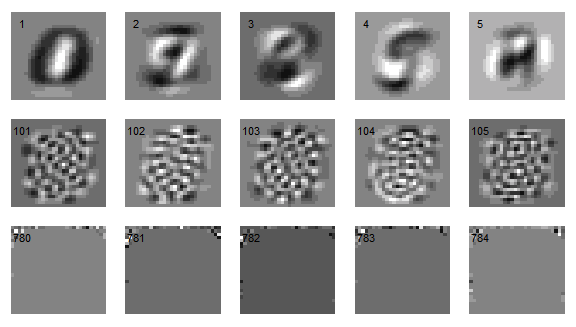
\includegraphics[width=0.75\textwidth]{pca_rotations_wider_range.png}}
\end{figure}

\begin{figure}[htb!]
\floatbox[{\capbeside\thisfloatsetup{capbesideposition={center,left},capbesidewidth=4.5cm}}]{figure}[\FBwidth]
{\caption{Cumulative amount of original variance kept as number of Principal Components (PCs) used increases. 87 PCs contain 90\% of the original data. Another 87 PCs increases this to 95.8\%.}\label{fig:cumsum_pca}}
{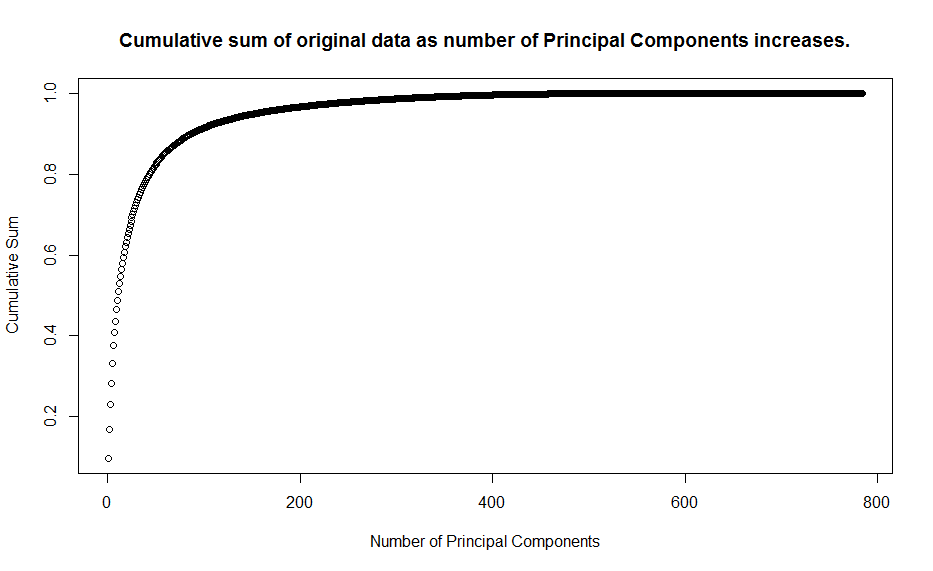
\includegraphics[width=0.6\textwidth]{cumulative_pca.png}}
\end{figure}

\vspace{-5mm}

Applying PCA before running a kNN algorithm should filter out noise, by reducing features to new properties with high variance, and reduce processing time, by reducing the number of variables to consider from 784, to a more reasonable amount.



\section{kNN}

\subsection{No preprocessing}

\subsubsection{First 10 Percent Training}

Initial classification attempts occurred with no dimensionality reduction, and instead just passed the first 6,000 training images, and the first 1,000 test images, into the kNN function. The MNIST dataset tends to get noisier, and less clear as the index increases, so while it should be good at classifiying the early images, it should struggle with later ones. 


\subsubsection{Random 10 Percent Training}

By taking instead a random sample of the training data, we can train our kNN on a more representative sample of the data. Again, 10\% of the training data is used, and the kNN is evaluated on both a random 10\% of the test data, and then the entirety of the test data. 

\begin{figure}[htb!]
\floatbox[{\capbeside\thisfloatsetup{capbesideposition={center,right},capbesidewidth=5cm}}]{figure}[\FBwidth]
{\caption{Comparison of different kNN training samples. Red is training and testing on first 10\% of respective data sets. Green is training and testing on random 10\% of respective data sets. Blue is training on random 10\% and testing on all test data.}\label{fig:init_kNN}}
{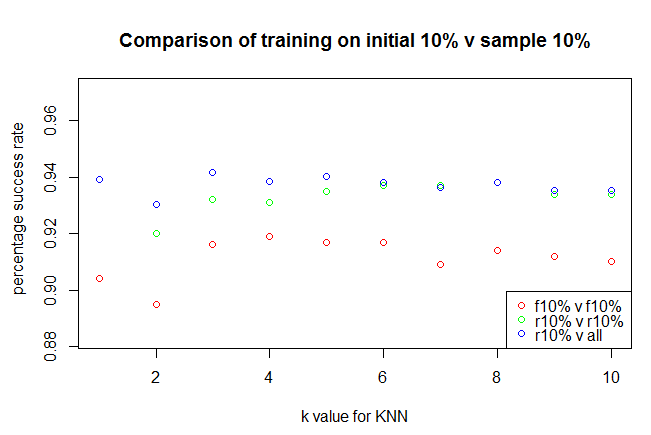
\includegraphics[width=0.6\textwidth]{10pc_training.png}}
\end{figure}



Figure \ref{fig:init_kNN} shows that the random 10\% sample tested on all data the highest success rate was from setting k to $3$, and yielded a success rate of 0.9415 - failing on only about 1 in 20 images. This is about 2\% higher on average than just taking the first 10\% of the training data. 





\subsection{PCA}

After applying principal component analysis, the kNN algorithm was run again, varying the number of PCs from 1 to 50, and varying the range of k values, from 1 to 17 in steps of 2. Figure \ref{fig:pca_rkvar} shows the first three plots for varying k values, showing success rates against both the training dataset of 6000 random images, and the test dataset of all 10,000 images. 

As expected, the training rate is always higher than the test rate, and for k = 1, the training rate is unsuprisingly 1 for every number of PCs used. As the number of PCs used increases, the success rate of the test data increases, until a plateau is reached after about 20 - 25 PCs. The plateaus for different k values sit at around the 0.973 $\pm$ 0.001 mark, with a max value of 0.9759 at k = 3, nPCs = 34. As k increases, the training success rate decreases, while the test success rate stays fairly consistant. 

\begin{figure}[htb!]
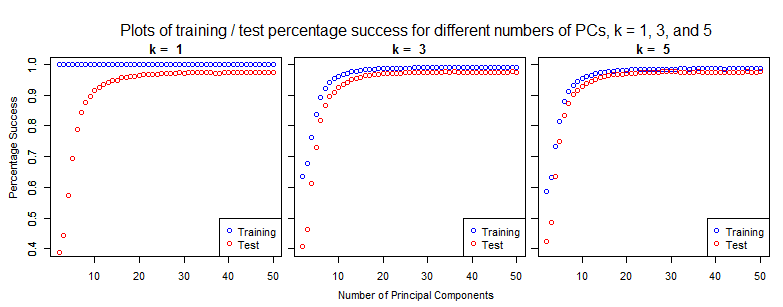
\includegraphics[width = 0.9\textwidth]{pca_kvar_traintest.png}
\caption{Comparison of training v test success rates for k values of 1, 3, and 5 as number of principal components used to trian with increases.} 
\label{fig:pca_rkvar}
\end{figure}




\section{Neural Networks}

A different method of classification is using a neural network. These are inspired by biological neurons in the brain, and offer huge scope for efficient classification. Unlike kNNs, it is not instance based, and so a model is created which allows for evaluating test data repeatedly with a single model - this reduces the need to hold all data in memory while classifying; once the model is created, it can be reused repeatedly with minimal memory costs - evaluating the entire set of test data takes a neglible amount of time once the network has been trained.

The algorithm works by building a network of weighted connectors, generating output values and a cost function (error between output and truth), and then propagating back through the network to update weights between the layers. This is iterated upon to reduce the cost function, until a minimum value is reached, or a maximum number of iterations is reached. 

First, the training data is normalised by dividing through by 255 (the maximum value of the greyscale array), and the labels are refactored into an array of boolean flags. The neural net is trained with a specific number of units in a hidden layer, for a defined number of iterations, before being used to predict output values with  a set of equally refactored test data. 

All neural networks were produced using the R function `nnet' which only allows a single hidden layer between the input and output layers. The output net is an $x \rightarrow y \rightarrow 10$ network, where $x$ is the number of principal components (the number of input variables), $y$ is the size of the hidden layer, which varies from 30 to 60 throughout the following work, and there are 10 possible output classifications (digits 0 to 9). 

\subsection{Initial Tests}


Neural Nets were trained with all 60,000 items of training data, and with other parameters varied as seen in Table \ref{nnet_parameters_init} in Appendix \ref{sec:AppNNetConfig}. This processing took approximately 24 hours (Windows 10, 12GB Ram, i5-4690k). Given the increase in correct classifications provided by preprocessing using PCA, all experiments were completed using the same PCA data as in the previous section.

The resulting data is summarised in the plots below. The results from the first plot, Figure \ref{fig:long_mean_nnet}, show an approximate 4\% increase in correct classification when increasing the number of iterations from 80 to 160, and a hidden layer size of 40 correctly classifies more digits than ones of 30 or 50. The second plot, Figure \ref{fig:long_mean_pc_nnet}, shows that for a hidden layer size of 40, there is only a small benefit gained from increasing the number of Principal Components used. 



\begin{figure}[htb!]
\floatbox[{\capbeside\thisfloatsetup{capbesideposition={center,left},capbesidewidth=4.5cm}}]{figure}[\FBwidth]
{\caption{A: Plot of average success rate against number of iterations. Size of hidden layer is depicted by line colour. Success rate is averaged over all principal component values.
B: Plot of average success rate against number of principal components used. Size of hidden layer is depicted by line colour. Success rate is averaged over all iterations from 110 onwards, reflecting the plateaued part of the percentage-iteration relationship.}\label{fig:long_mean_nnet}}
{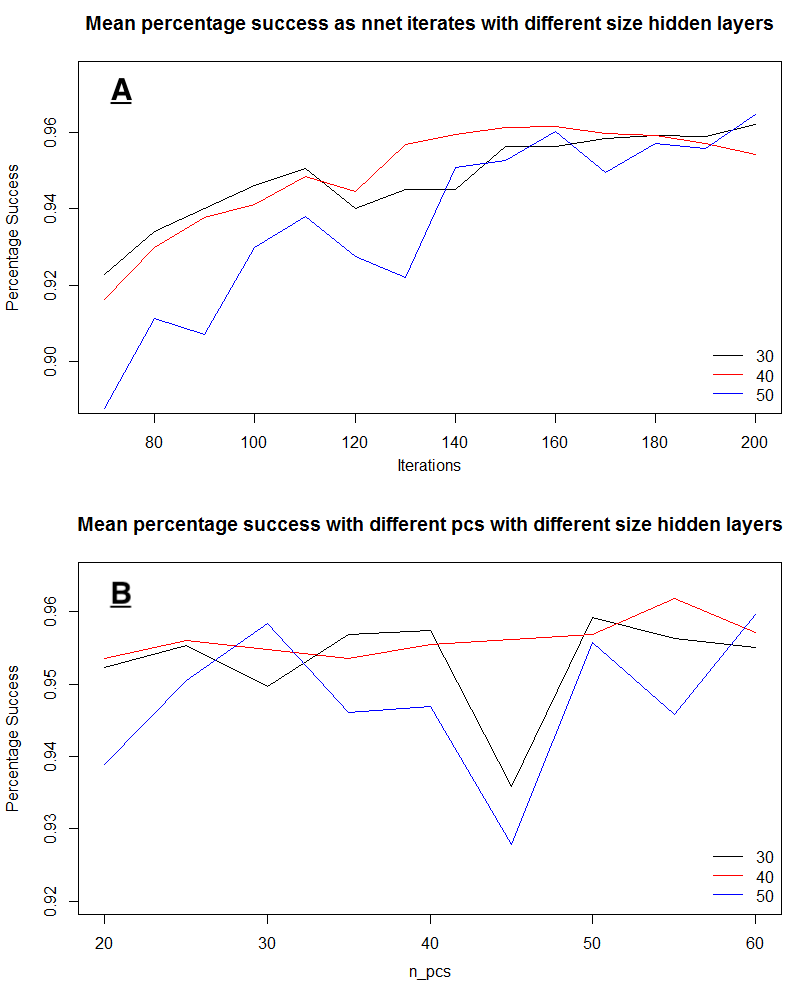
\includegraphics[width=0.55\textwidth]{long_mean_it_dupe.png}}
\end{figure}

%
%\begin{figure}[htb!]
%\floatbox[{\capbeside\thisfloatsetup{capbesideposition={center,left},capbesidewidth=4cm}}]{figure}[\FBwidth]
%{\caption{Plot of average success rate against number of iterations. Size of hidden layer is depicted by line colour. Success rate is averaged over all principal component values.}\label{fig:long_mean_nnet}}
%{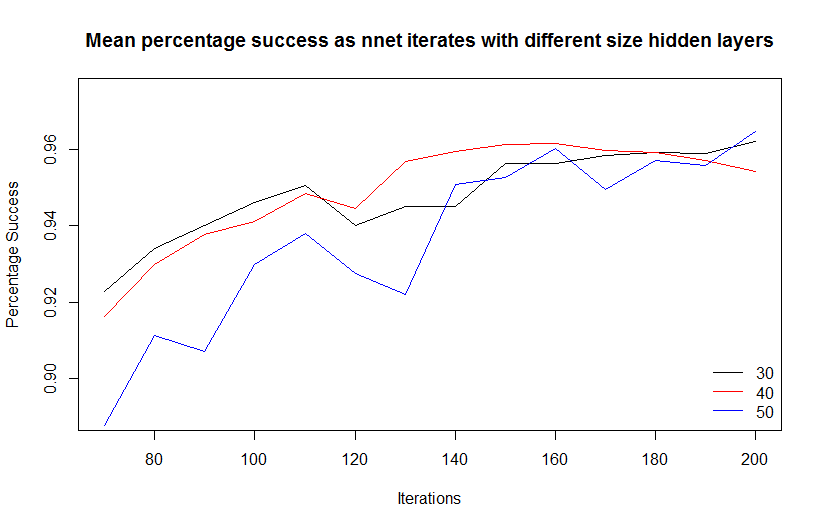
\includegraphics[width=0.6\textwidth]{long_mean_it.png}}
%\end{figure}
%
%\begin{figure}[htb!]
%\floatbox[{\capbeside\thisfloatsetup{capbesideposition={center,right},capbesidewidth=4.5cm}}]{figure}[\FBwidth]
%{\caption{Plot of average success rate against number of principal components used. Size of hidden layer is depicted by line colour. Success rate is averaged over all iterations from 110 onwards, reflecting the plateaued part of the percentage-iteration relationship.}\label{fig:long_mean_pc_nnet}}
%{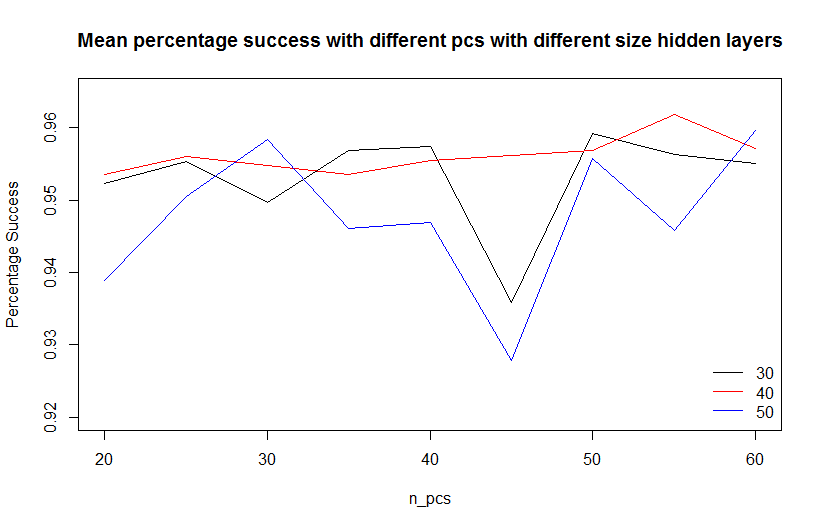
\includegraphics[width=0.6\textwidth]{long_mean_pcs_cutdown.png}}
%\end{figure}

\subsection{Secondary Tests - Extended Iterations, Hidden Layer}

Given the initial tests showed that the success rate increases with the number of iterations, secondary tests extending the number of iterations to 500 were completed. As seen in Table \ref{nnet_parameters_second} within Appendix \ref{sec:AppNNetConfig}, neural nets were created with hidden layers from 40 to 60, with a smaller resolution of principal components to vary over, but going up to a higher value (70 rather than 60). Instead of iterating between 70 and 200 times, it iterates from 120 to 500. Again, this took approximately 24 hours - despite the reduced number of variables to try, the higher iterations unsuprisingly take a lot longer. 

Figure \ref{fig:ext_mean_nnet} shows the plateauing nature of increasing the number of iterations, while Figure \ref{fig:ext_mean_pc_nnet} shows the small effect of increasing the number of PCs used. 

\begin{figure}[htb!]
\floatbox[{\capbeside\thisfloatsetup{capbesideposition={center,left},capbesidewidth=4cm}}]{figure}[\FBwidth]
{\caption{Plot of average success rate against number of iterations. Size of hidden layer is depicted by line colour. Success rate is averaged over all principal component values. }\label{fig:ext_mean_nnet}}
{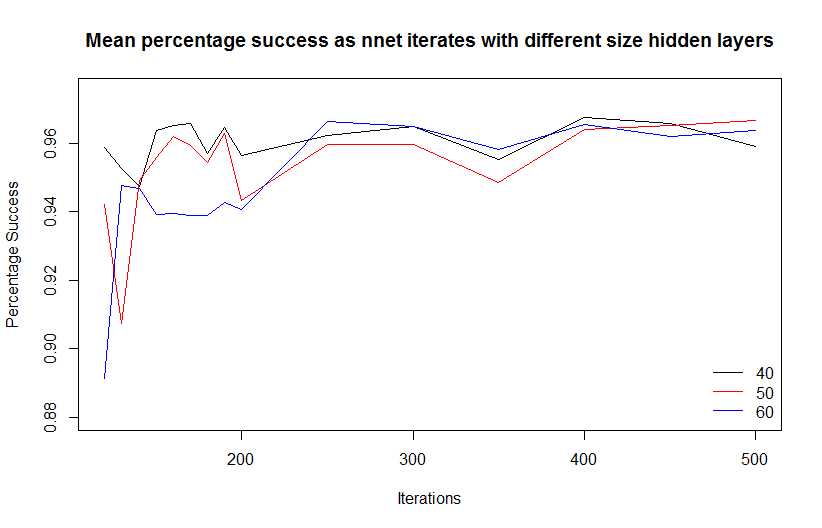
\includegraphics[width=0.6\textwidth]{nnet_extend_iter_mean.png}}
\end{figure}

\begin{figure}[htb!]
\floatbox[{\capbeside\thisfloatsetup{capbesideposition={center,right},capbesidewidth=4.5cm}}]{figure}[\FBwidth]
{\caption{Plot of average success rate against number of principal components used. Size of hidden layer is depicted by line colour. Success rate is averaged over all iterations from 160 onwards.}\label{fig:ext_mean_pc_nnet}}
{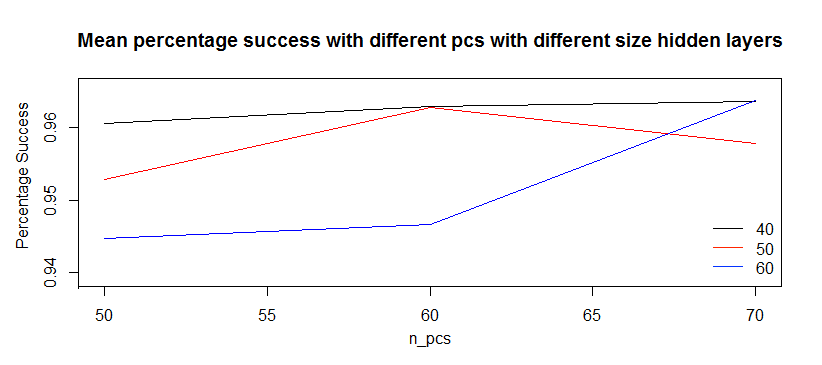
\includegraphics[width=0.6\textwidth]{nnet_mean_diff_pcs_extended_it2.png}}
\end{figure}

The highest success rate for 10,000 test images occurred with a 70-40-10 neural net, iterating 190 times, and yielded a 0.9692 success rate. 

\subsection{Tertiary Tests, Extended Iterations}

For the third set of tests, the size of the hidden layer was set to 40 for each neural net produced. Up to 3000 iterations were used, extending greatly the range used in previous trials. The number of principal components used varied from 50 to 150, again, reaching almost double the amount previously used.


\begin{figure}[htb!]
\floatbox[{\capbeside\thisfloatsetup{capbesideposition={center,left},capbesidewidth=5.5cm}}]{figure}[\FBwidth]
{\caption{Plot of success rate against number of iterations for different principal components used. A hidden layer of size 40 was used. Increasing the number of principal components beyond 50 has a negative effect on the number of images correctly identified. }\label{fig:superext_nnet}}
{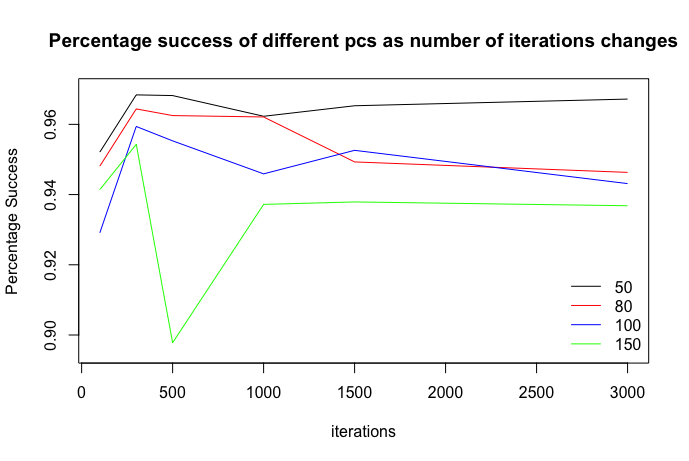
\includegraphics[width=0.5\textwidth]{nn_superext.png}}
\end{figure}

Beyond a certain point - around 500 iterations - there is a general decrease in percentage success. The highest success rate for 10,000 test images occurred with a 50-40-10 neural net, iterating 300 times, and yielded a 0.9684 success rate.


\section{Analysis}

Both the classification methods used above yield similar maximum success rates. Applying a kNN to PCAd data, yielded a success rate of 0.9759 with k = 3, and using 34 PCs. Meanwhile, with a 50-40-10 neural net iterated 300 times, a 0.9684 success rate, approximately 1 \% lower. 

While the kNN was more successful, the algorithm is very simple and has little scope for improving. Whereas neural networks offer far more in the way of fine tuning and altering of parameters; adding more hidden layers (beyond the scope of the functions used), using convolutional neural networks (CNN) or other more complicated neural networks. Examples of other algorithm success rates can be found at \cite{mnist-website}. However, the functionality of the two methods is different. The neural net provides a model which can be used repeatedly to test images, allowing the processing-intensive work to be done on a powerful workstation, while the classification of new images can happen very rapidly on a much less powerful machine. The kNN however evaluates against the entirety of the training set for every image, and no model can be built ahead of time to save on processing. 

\section{Conclusion}

Both methods provide similarly high classification rates, failing on only 2-3\% of images, once PCA has been applied to the data. While kNN yielded a higher rate, it is a much slower algorithm to run, and offers very little in the way of parameter tuning compared to the neural network method. Extra preprocessing could be attempted, to remove pixels of low variance before applying PCA which might allow minor improvements in the success rate, or in the case of the neural network, using multiple interconnected hidden layers with different activation functions could be explored to increase performance. 

\newpage
\begin{thebibliography}{9}



\bibitem{mnist-website} MNIST overview, \url{yann.lecun.com/exdb/mnist}, Accessed 2019-04-02

\end{thebibliography}

\appendix
\label{appendix}
%\section{Summary Data for kNN}
%\label{sec:AppData}

%\begin{table}[h]
%\begin{center}
%\begin{tabular}{l| c c c c c c c c c c}
% & 1 & 2 & 3 & 4 & 5 & 6 & 7 & 8 & 9 & 10\\
%\hline
%A & 0.904 & 0.895 & 0.916 & 0.919 & 0.917 & 0.917 & 0.909 & 0.914 & 0.912 & 0.910\\
%B & 0.939 & 0.920 & 0.932 & 0.931 & 0.935 & 0.937 & 0.937 & 0.938 & 0.934 & 0.934\\
%C & 0.9390 & 0.9303 & 0.9415 & 0.9383 & 0.9401 & 0.9381 & 0.9362 & 0.9380 & 0.9352 & 0.9354\\
%\end{tabular}
%\caption{Success rates for $k = 1:10$. A: trained on 6,000 random digits and tested on random 1,000 digits (Red in Fig \ref{fig:init_kNN}). B: trained on 6,000 random digits and tested on random 1,000 digits (Green in Fig \ref{fig:init_kNN}). C: trained on 6,000 random digits and tested on all 10,000 digits (Blue in Fig \ref{fig:init_kNN}).}
%\label{rand-10-all-test}
%\end{center}
%\end{table}

%\section{PCA for kNN}
%\label{sec:App_PCA}
%
%\begin{figure}[htb!]
%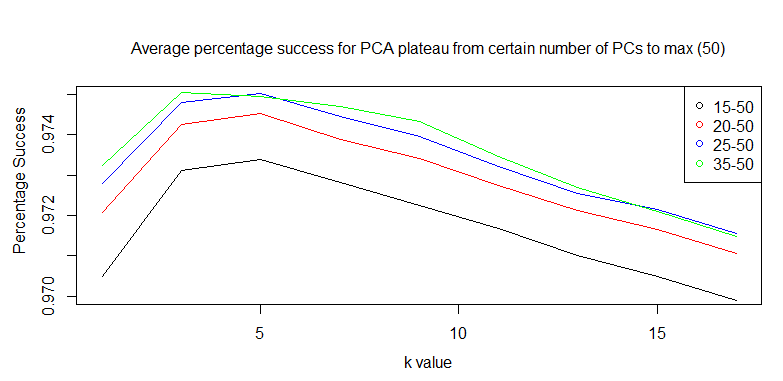
\includegraphics[width = 0.9\textwidth]{pca_knn_avplateau.png}
%\caption{Shows the average percentage success for the plateaued part of the curve, from defined numbers of principal components. By the 25th PC, the success rate has stopped increasing rapidly - as shown in comparison with the green line for 35 PCs.} 
%\label{fig:pca_kNN_avplateau}
%\end{figure}

\section{Neural Network configurations}
\label{sec:AppNNetConfig}

\begin{table}[h!]
\begin{center}
\begin{tabular}{rl}
Parameter & Values \\
\hline
Hidden Layer Size & 30, 40, 50\\
Number of PCs & 20, 25, 30, 35, 40, 45, 50, 55, 60\\
Neural Net Iterations & 70, 80, 90, 100, 110, 120, 130,\\
& 140, 150, 160, 170, 180, 190, 200\\
\hline
\end{tabular}
\caption{Configuration values for initial Neural Network tests.}
\label{nnet_parameters_init}
\end{center}
\end{table}


\begin{table}[h!]
\begin{center}
\begin{tabular}{rl}
Parameter & Values \\
\hline
Hidden Layer Size & 40, 50, 60\\
Number of PCs & 50, 60, 70\\
Neural Net Iterations &  120, 130, 140, 150, 160, 170, 180, 190,\\
& 200, 250, 300, 350, 400, 450, 500\\
\hline
\end{tabular}
\caption{Configuration values for secondary Neural Network tests.}
\label{nnet_parameters_second}
\end{center}
\end{table}


\begin{table}[h!]
\begin{center}
\begin{tabular}{rl}
Parameter & Values \\
\hline
Hidden Layer Size & 40\\
Number of PCs & 50, 80, 100, 150\\
Neural Net Iterations & 100, 300, 500, 1000, 1500, 3000\\
\hline
\end{tabular}
\caption{Configuration values for tertiary Neural Network tests.}
\label{nnet_parameters_third}
\end{center}
\end{table}


\section{Source Code}

Section \ref{code-input} contains a slightly modified version of the input-data script provided. 

Section \ref{code-general} contains several functions used throughout for running kNNs and evaluating their success rate.

Section \ref{code-vars} contains code needed to set up the workspace, input required data, and preprocess with PCA.

Section \ref{code-knn} contains all the code for the kNN examples found above.

Section \ref{code-nnet} contains the code for the neural network work found above.

\subsection{Input Data}
\label{code-input}

Functions provided during course, `load\_mnist' function edited to take input paths. 
\begin{lstlisting}

# Load the MNIST digit recognition dataset into R
# http://yann.lecun.com/exdb/mnist/
# assume you have all 4 files and gunzip'd them
# creates train$n, train$x, train$y  and test$n, test$x, test$y
# e.g. train$x is a 60000 x 784 matrix, each row is one digit (28x28)
# call:  show_digit(train$x[5,])   to see a digit.
# brendan o'connor - gist.github.com/39760 - anyall.org
load_mnist <- function(train.path = 'data/train-images.idx3-ubyte',
                       test.path = 'data/t10k-images.idx3-ubyte',
                       train.labels.path = 'data/train-labels.idx1-ubyte',
                       test.labels.path = 'data/t10k-labels.idx1-ubyte') {
  load_image_file <- function(filename) {
    ret = list()
    f = file(filename,'rb')
    readBin(f,'integer',n=1,size=4,endian='big')
    ret$n = readBin(f,'integer',n=1,size=4,endian='big')
    nrow = readBin(f,'integer',n=1,size=4,endian='big')
    ncol = readBin(f,'integer',n=1,size=4,endian='big')
    x = readBin(f,'integer',n=ret$n*nrow*ncol,size=1,signed=F)
    ret$x = matrix(x, ncol=nrow*ncol, byrow=T)
    close(f)
    ret
  }
  load_label_file <- function(filename) {
    f = file(filename,'rb')
    readBin(f,'integer',n=1,size=4,endian='big')
    n = readBin(f,'integer',n=1,size=4,endian='big')
    y = readBin(f,'integer',n=n,size=1,signed=F)
    close(f)
    y
  }
  train <<- load_image_file(train.path)
  test <<- load_image_file(test.path)
  
  train$y <<- load_label_file(train.labels.path)
  test$y <<- load_label_file(test.labels.path)  
}

show_digit <- function(arr784, col=gray(12:1/12), ...) {
  image(matrix(arr784, nrow=28)[,28:1], col=col, ...)
}

\end{lstlisting}

\subsection{General functions}
\label{code-general}

Contains general functions used to run kNN on sets of data, and assess the results against truth values.

\begin{lstlisting}


run_knn <- function(train.data, train.labels, test.data, test.labels, k.range, 
                    to.console = TRUE,to.file = FALSE, filepath = "") {
  ### Performs n knns and returns a copy of the results.
  ### Runs with a range of different k values as specified by k.range
  ### Inputs:
  ###   train.data - Matrix of m rows and n columns. Each row is an observation 
  ###                for the knn, while each column is a variable
  ###   train.labels - Array of labels for the training data. Should be of dim 
  ###                  1xm, one value for each observation
  ###   test.data - Matrix of p rows and n columns. As with training data, each 
  ###               row is an observation, each column a variable
  ###   test.labels - Array of labels for the test data of dim 1xp. Only used if 
  ###                 to.console is set to TRUE
  ###   k.range - iterable, range of k values to run the knn with.
  ###   to.console - Boolean, whether to print out k values and percentage 
  ###                success to console.
  ###   to.file - Boolean, whether to print to a file or not. If TRUE,  
  ###             file.path must be specified.
  ###   file.path - Str, path of location to write CSV output to. Will write  
  ###               after each knn has been classified.  
  ###
  ### Outputs:
  ###   results.full - Output Matrix of x rows and p columns, where x is the  
  ###                  length of k.range. Each row contains the results for a 
  ###                  specific k value.
  ###                - Each column contains the predicted label for that index of 
  ###                  test data. 

  if (to.file & is.empty(filepath)){
    stop("Unable to write to a file without a filepath specified.")
  }
  
  #build results matrix
  results.full <- matrix(0,nrow = length(k.range), ncol = length(test.labels))

  it <- 1
  for (k in k.range){
    #run KNN and store in matrix. 
    results <- knn(train = train.data, 
                   test = test.data, 
                   cl = train.labels, 
                   k = k)
    
    results.full[it,] <- results
    
    if (to.file){
      write.csv(results.full, file = filepath, append = FALSE)
    }
    
    #print percentage results to console if set
    if(to.console){
      correct <- results == test.labels
      perc <- sum(correct)/length(correct) 
      print(c(k, perc))
    }
    
    it <- it + 1
  }
  
  return(results.full)
}


assess_knn <- function(expected, found){
  ### Compares expected values to calculated values and provides a percentage 
  ### value for each, 
  ###
  ### Inputs:
  ###   expected - 1xp array of correct labels for Test data set.
  ###   found - nxp matrix of predicted labels for Test data set. The number 
  ###           of rows, n, is the number of different models used to loop over.
  ###
  ### Outputs:
  ###   percentages - 
  
  #build results array
  percentages <- array(0, nrow(found))
  
  for (k in 1:nrow(found)){
    #for each row of the found matrix, compare to correct. 
    #'-1' needed as 1 is added to every value in found matrix due to issue with  
    #0 as a classification output
    correct <- expected == found[k,] - 1
    percentages[k] <- sum(correct)/length(correct)
  }
  
  return(percentages)
}

\end{lstlisting}

\subsection{Set up variables}
\label{code-vars}

Below code should be run before any following set of code. Imports necessary packages, sets directory, imports data, performs PCA, and plots the first 3 plots. 

\begin{lstlisting}

library(class)
library(tictoc)
library(nnet)
library(rapportools)
wd <- "/Users/training2/Desktop/ML-R"
output <- "./data/"
setwd(wd)

source("load_MNISTR.R")
source("run_knn.R")

### Default paths for files from WD. Uncomment and respecify path 
### to override defaults in load_mnist() 
# train.path <- 'data/train-images.idx3-ubyte'
# test.path <-  'data/t10k-images.idx3-ubyte'
# train.labels.path <-  'data/train-labels.idx1-ubyte'
# test.labels.path <-  'data/t10k-labels.idx1-ubyte'

### Set seed for sample reproducability
set.seed(11235813)

sample.10pc <- sample(1:60000,6000)
sample.test10pc <- sample(1:10000,1000)

### Load in Training, Test, and Label Files.
load_mnist()

### Plot first digit 
show_digit(train$x[1,])



### Set seed for reproducability
set.seed(11235813)

### Run PCA on the training data - all of it, apply to test data,
full.pca <- prcomp(train$x,center = TRUE)
train.pca <- full.pca$x
test.pca <- predict(full.pca, test$x)

###Find cumulative sum of retained data, plot
cs <- cumsum(full.pca$sdev^2 / sum(full.pca$sdev^2))
plot(cs, ylab = 'Cumulative Sum', xlab = 'Number of Principal Components', 
	main = paste('Cumulative sum of original data as', 
	'number of Principal Components increases'))

###Plot first 3 components, 101 to 105, and 780 to 784 in 3x5 array
par(mfrow = c(3,5), mai = c(0.1,0.1,0.1,0.1))
for (i in c(1:5, 101:105, 780:784)){
  show_digit(full.pca$rotation[,i],axes=FALSE,xlab="",ylab="",srt=45)
  text(0.1,0.9, i)
}
\end{lstlisting}


\subsection{kNN}
\label{code-knn}
\subsubsection{Initial kNN}
\label{code-init_knn}

Below code runs the initial kNN analysis with no preprocessing. 

\begin{lstlisting}

### Run KNN for first 10% of both training and test data set, for k = 1:10
k.range.initial10 <- c(1:10)
fp <- paste(output,"init10pc10k.csv",sep=""))
full.results.initial10 <- run_knn(train$x[1:6000,], 
                                      train$y[1:6000], 
                                      test$x[1:1000,], 
                                      test$y[1:1000], 
                                      k.range.initial10,
                                      to.console = FALSE,
                                      to.file = TRUE,
                                      filepath = fp

percentages.initial10 <- assess_knn(test$y[1:1000], full.results.initial10)


### Run KNN on a random 10% of training, and random 10% of test set, for k = 1:10

k.range.random10 <- c(1:10)
fp <- paste(output,"rand10pc10k.csv",sep=""))
full.results.random10_10 <- run_knn(train$x[sample.10pc,], 
                                        train$y[sample.10pc], 
                                        test$x[sample.test10pc,], 
                                        test$y[sample.test10pc], 
                                        k.range.random10,
                                        to.console = FALSE,
                                        to.file = TRUE,
                                        filepath = f[

percentages.random10_10 <- assess_knn(test$y[sample.test10pc], 
	full.results.random10_10)


### Run KNN on a random 10% of training, and the whole test set, for k = 1:10

k.range.random10 <- c(1:10)
fp <- paste(output,"rand10full10k.csv",sep=""))
full.results.random10_all <- run_knn(train$x[sample.10pc,], 
                                         train$y[sample.10pc], 
                                         test$x, 
                                         test$y, 
                                         k.range.random10,
                                         to.console = FALSE,
                                         to.file = TRUE,
                                         filepath = fp

percentages.random10_all <- assess_knn(test$y, full.results.random10_all)

### plot first 10% training, 10% test against rand 10% train, rand 10% test, 
### against rand 10%train, all test 
windows()
plot(1:10, percentages.initial10, col = "red",ylim=c(0.85,0.97),
	main="Comparison of training on initial 10% v sample 10%", 
	xlab="k value for KNN", 
	ylab ="percentage success rate at classifying (%)")
points(1:10, percentages.random10_10, col = "green")
points(1:10, percentages.random10_all, col = "blue")
legend("bottomright", 
	legend = c("f10% v f10%", "r10% v r10%","r10% v all"), 
	col = c("red", "green","blue"), pch = 1)


\end{lstlisting}
\vspace{15mm}
\subsubsection{kNN on PCA}
\label{code-pca_knn}

Below code runs kNN on data that has had PCA applied to it. 

\begin{lstlisting}

upper.bounds <- 2:50
k.range <- seq(1,17,2)
results.train.default <- matrix(0, ncol = length(upper.bounds), 
	nrow = length(k.range))
results.test.default <- matrix(0, ncol = length(upper.bounds), 
	nrow = length(k.range))
for (k in k.range){
  # results.train <- c()
  # results.test <- c()
  for (upper.bound in upper.bounds){
    pca.to.use <- 1:upper.bound
    predict.train <- knn(train = train.pca[sample.idx,pca.to.use], 
                         test = train.pca[sample.idx,pca.to.use],
                         cl = train$y[sample.idx],
                         k = k)
    correct <- predict.train == train$y[sample.idx]
    results.train.default[k,upper.bound - 1] <- (sum(correct)/length(correct))
    # print(sum(correct)/length(correct))
    predict.test <- knn(train = train.pca[sample.idx,pca.to.use], 
                        test = test.pca[,pca.to.use],
                        cl = train$y[sample.idx],
                        k = k)
    correct <- predict.test == test$y
    results.test.default[k,upper.bound - 1] <- (sum(correct)/length(correct))
  }
  
par(mfrow = c(1,3), oma = c(4,4,3,0.1), mar = c(0,0,1.5,1))
for (k in k.range[1:3]){  
  #windows()
  if (k == 1){ 
    plot(upper.bounds, results.train.default[(k/2)+0.5,], 
	col = "blue", ylim=c(0.4,1), 
         main = paste('k = ', k), 
	xlab = "number of PCs", 
	ylab = "percentage success")
  } else {
    plot(upper.bounds, results.train.default[(k/2)+0.5,], 
	col = "blue", ylim=c(0.4,1), 
         main = paste('k = ', k), 
	xlab = "number of PCs", yaxt = "n")
  }
  points(upper.bounds, results.test.default[(k/2)+0.5,], col = "red")
  axis(side = 2, labels = k == 1)
  
  legend("bottomright", 
	legend = c("Training","Test"), 
	col = c("blue", "red"), pch = 1)
}
title(xlab = 'Number of Principal Components', 
      ylab = 'Percentage Success',
      outer = TRUE, line = 2.5)
mtext(paste('Plots of training / test percentage success for different', 
	    'numbers of PCs, k = 1, 3, and 5'), 
      outer = TRUE, cex = 1)


\end{lstlisting}

\subsection{Neural Networks}
\label{code-nnet}

\subsubsection{Initial Neural Network}
\label{code-init_nnet}
\begin{lstlisting}

#assumes that PCA has been done elsewhere. 
#Takes about 24 hours to complete

set.seed(11235813)
mx <- max(train.pca)
mn <- min(train.pca)
#can't normalise by dividing by max, as range of values is not 0 - 255, 
#but between a large negative and large positive number. 
#Instead, normalise by (x - min)/(max - min) which will convert to range 0 to 1
test.data <- (test.pca - mn) / (mx - mn) 

training.labels <- t(t(train$y))
training.label <- as.factor(training.labels)

#nnet requires a boolean array of labels
Y <- class.ind(training.label)

n_pcs_seq <- seq(20,60,5)
it_seq <- seq(70,200,10)
sz_seq <- seq(30,50,10)
n_train <- 60000

#initialise output vector
results.train <- array(rep(0, length(n_pcs_seq) * length(it_seq) * length(sz_seq)),
                       c(length(n_pcs_seq), length(it_seq), length(sz_seq)))

for (sz in sz_seq){
  for (n_pcs in n_pcs_seq){
    training.data <- (train.pca[,c(1:n_pcs)] - mn) / (mx - mn)
    for (it in it_seq){
      nn <- nnet(training.data, Y, size = sz, maxit = it, MaxNWts = 50000, 
           softmax = TRUE)
      
      z <- predict(nn, test.data, type='class')
      correct <- z == test$y
      perc <- sum(correct) / length(correct)
      
      
      r <- (n_pcs / 5) - (n_pcs_seq[1] / 5 - 1) 
      c <- (it / 10) - (it_seq[1] / 10 - 1)
      d <- (sz / 10) - (sz_seq[1] / 10 - 1)
      
      results.train[r,c,d] <- perc
      
      cat(sz, n_pcs, it, n_train, perc, '\n', file = "log.txt", append=TRUE)
      
    }
  }
}


plot(it_seq, apply(results.train[,,1], MARGIN = 2, mean), pch = 0, 
     xlab = 'Iterations', ylab='Percentage Success', 
     main = paste('Mean percentage success as nnet ', 
          'iterates with different size hidden layers'), 
     type = 'l', ylim = c(0.89,0.975))
lines(it_seq, apply(results.train[,,2], MARGIN = 2, mean), col = 'red')
lines(it_seq, apply(results.train[,,3], MARGIN = 2, mean), col = 'blue')
legend(x = 'bottomright', legend = c('30','40','50'), 
       col = c('black','red','blue'), bty = 'n', lty = c(1,1,1))

#plots max value rather than mean. Not featured in report.
#plot(it_seq, apply(results.train[,,1], MARGIN = 2, max), pch = 0, 
#     xlab = 'Iterations', ylab='Percentage Success', 
#     main = paste('Max percentage success as nnet ', 
#          'iterates with different size hidden layers'), 
#     type = 'l', ylim = c(0.92,0.975))
#lines(it_seq, apply(results.train[,,2], MARGIN = 2, max), col = 'red')
#lines(it_seq, apply(results.train[,,3], MARGIN = 2, max), col = 'blue')
#legend(x = 'bottomright', legend = c('30','40','50'), 
#       col = c('black','red','blue'), bty = 'n', lty = c(1,1,1))

#plots for all iterations, rather than for plateau
#plot(n_pcs_seq, apply(results.train1[,,1], MARGIN = 1, mean), pch = 0, 
#     xlab = 'n_pcs', ylab='Percentage Success', 
#     main = paste('Mean percentage success with different pcs',
#          ' with different size hidden layers'), 
#     type = 'l', ylim = c(0.92,0.96))
#lines(n_pcs_seq, apply(results.train[,,2], MARGIN = 1, mean), col = 'red')
#lines(n_pcs_seq, apply(results.train[,,3], MARGIN = 1, mean), col = 'blue')
#legend(x = 'bottomright', legend = c('30','40','50'), 
#       col = c('black','red','blue'), bty = 'n', lty = c(1,1,1))

#5:14 chosen as plateau of iteration shelf
plot(n_pcs_seq, apply(results.train[,5:14,1], MARGIN = 1, mean), pch = 0, 
     xlab = 'n_pcs', ylab='Percentage Success', 
     main = paste('Mean percentage success with different pcs',
          ' with different size hidden layers'), 
     type = 'l', ylim = c(0.92,0.965))
lines(n_pcs_seq, apply(results.train[,5:14,2], MARGIN = 1, mean), col = 'red')
lines(n_pcs_seq, apply(results.train[,5:14,3], MARGIN = 1, mean), col = 'blue')
legend(x = 'bottomright', legend = c('30','40','50'), 
       col = c('black','red','blue'), bty = 'n', lty = c(1,1,1))

\end{lstlisting}

\vspace{5mm}
\subsubsection{Secondary Neural Network}
\label{code-sec_nnet}


\begin{lstlisting}
#assumes that PCA has been done elsewhere. 
#extended nnet for higher value iterations - about 24 hours

set.seed(11235813)

training.labels <- t(t(train$y))
training.label <- as.factor(training.labels)

Y <- class.ind(training.label)

n_train <- 60000
n_pcs_seq <- seq(50,70,10)
it_seq <- c(120,130,140,150,160,170,180,190,200,250,300,350,400,450,500)
sz_seq <- seq(40,60,10)

results.train <- array(rep(0, length(n_pcs_seq) * length(it_seq) * length(sz_seq)),
                       c(length(n_pcs_seq), length(it_seq), length(sz_seq)))

best_nn_perc <- 0

for (sz in sz_seq){
  for (n_pcs in n_pcs_seq){
    #normalise training data
    mx <- max(train.pca)
    mn <- min(train.pca)
    training.data <- (train.pca[,c(1:n_pcs)] - mn) / (mx - mn)
    test.data <- (test.pca - mn) / (mx - mn)
    
    it_iterator <- 0
    for (it in it_seq){
      it_iterator <- it_iterator + 1
      
      nn <- nnet(training.data, Y, size = sz, maxit = it, 
                 MaxNWts = 50000, softmax = TRUE)
      
      z <- predict(nn, test.data, type='class')
      correct <- z == test$y
      perc <- sum(correct) / length(correct)
      
      r <- (n_pcs / 10) - (n_pcs_seq[1] / 10 - 1)
      c <- it_iterator
      d <- (sz / 10) - (sz_seq[1] / 10 - 1)
      
      results.train[r,c,d] <- perc
      cat(sz, n_pcs, it, n_train, perc, '\n', file = "log.txt", append=TRUE)
      
      
      if (perc > best_nn_perc){
        best_nn_perc <- perc
        cat(sz, n_pcs, it, n_train, perc, '\n', file = "log_best.txt", append=TRUE)
        best_nn <- nn
        best_it <- it
        best_pc <- n_pcs
        best_sz <- sz
      }
    }
  }
}


plot(it_seq, apply(results.train[,,1], MARGIN = 2, mean), pch = 0, 
     xlab = 'Iterations', ylab='Percentage Success', 
     main = paste('Mean percentage success as nnet iterates',
                  ' with different size hidden layers'), 
     type = 'l', ylim = c(0.925,0.975))
lines(it_seq, apply(results.train[,,2], MARGIN = 2, mean), col = 'red')
lines(it_seq, apply(results.train[,,3], MARGIN = 2, mean), col = 'blue')
legend(x = 'bottomright', legend = c('40','50','60'), 
       col = c('black','red','blue'), bty = 'n', lty = c(1,1,1))

plot(n_pcs_seq, apply(results.train[,,1], MARGIN = 1, mean), pch = 0, 
     xlab = 'n_pcs', ylab='Percentage Success', 
     main = paste('Mean percentage success with different ',
                  'pcs with different size hidden layers'), 
     type = 'l', ylim = c(0.92,0.96))
lines(n_pcs_seq, apply(results.train[,,2], MARGIN = 1, mean), col = 'red')
lines(n_pcs_seq, apply(results.train[,,3], MARGIN = 1, mean), col = 'blue')
legend(x = 'bottomright', legend = c('40','50','60'), 
       col = c('black','red','blue'), bty = 'n', lty = c(1,1,1))

#5:14 chosen as plateau of iteration shelf
plot(n_pcs_seq, apply(results.train[,5:14,1], MARGIN = 1, mean), pch = 0, 
     xlab = 'n_pcs', ylab='Percentage Success', 
     main = paste('Mean percentage success with different ',
                  'pcs with different size hidden layers'), 
     type = 'l', ylim = c(0.92,0.965))
lines(n_pcs_seq, apply(results.train[,5:14,2], MARGIN = 1, mean), col = 'red')
lines(n_pcs_seq, apply(results.train[,5:14,3], MARGIN = 1, mean), col = 'blue')
legend(x = 'bottomright', legend = c('40','50','60'), 
       col = c('black','red','blue'), bty = 'n', lty = c(1,1,1))


\end{lstlisting}

\vspace{5mm}

\subsubsection{Tertiary Neural Network}
\label{code-tert_nnet}

\begin{lstlisting}

#assumes that PCA has been done elsewhere. 
#extended nnet for higher value iterations - about 24 hours

set.seed(11235813)

training.labels <- t(t(train$y))
training.label <- as.factor(training.labels)

Y <- class.ind(training.label)

n_train <- 60000
n_pcs_seq <- c(50, 80, 100, 150)
it_seq <- c(100, 300, 500, 1000, 1500, 3000)
sz_seq <- c(40)

results.train <- array(rep(0, length(n_pcs_seq) * length(it_seq) * length(sz_seq)),
                       c(length(n_pcs_seq), length(it_seq), length(sz_seq)))

best_nn_perc <- 0

for (sz in sz_seq){
  npc_iterator <- 0 
  for (n_pcs in n_pcs_seq){
    npc_iterator <- npc_iterator + 1
    
    #normalise training data
    mx <- max(train.pca)
    mn <- min(train.pca)
    training.data <- (train.pca[,c(1:n_pcs)] - mn) / (mx - mn)
    test.data <- (test.pca - mn) / (mx - mn)
    
    it_iterator <- 0
    for (it in it_seq){
      it_iterator <- it_iterator + 1
      
      nn <- nnet(training.data, Y, size = sz, maxit = it, 
                 MaxNWts = 50000, softmax = TRUE)
      
      z <- predict(nn, test.data, type='class')
      correct <- z == test$y
      perc <- sum(correct) / length(correct)
      
      r <- npc_iterator
      c <- it_iterator
      d <- 1
      
      results.train[r,c,d] <- perc
      cat(sz, n_pcs, it, n_train, perc, '\n', 
          file = "log_e.txt", append=TRUE)
      
      
      if (perc > best_nn_perc){
        best_nn_perc <- perc
        cat(sz, n_pcs, it, n_train, perc, '\n', 
            file = "log_e_best.txt", append=TRUE)
        best_nn <- nn
        best_it <- it
        best_pc <- n_pcs
        best_sz <- sz
      }
    }
  }
}

#plot results

plot(it_seq, results.train[1,,1], pch = 0, xlab = 'iterations', ylab = 'Percentage Success', 
     main = 'Percentage success of different pcs as number of iterations changes',
     type = 'l', ylim = c(0.895, 0.97))
lines(it_seq, results.train[2,,1], col = 'red')
lines(it_seq, results.train[3,,1], col = 'blue')
lines(it_seq, results.train[4,,1], col = 'green')
legend(x = 'bottomright', legend = c('50','80','100','150'), 
       col = c('black','red','blue','green'), bty = 'n', 
       lty = c(1,1,1,1))




\end{lstlisting}

\end{document}
